\hypertarget{_example_c_p_p_federate_8cpp}{
\section{ExampleCPPFederate.cpp File Reference}
\label{_example_c_p_p_federate_8cpp}\index{ExampleCPPFederate.cpp@{ExampleCPPFederate.cpp}}
}
{\ttfamily \#include $<$iostream$>$}\par
{\ttfamily \#include $<$memory.h$>$}\par
{\ttfamily \#include \char`\"{}ExampleFedAmb.h\char`\"{}}\par
{\ttfamily \#include \char`\"{}ExampleCPPFederate.h\char`\"{}}\par
{\ttfamily \#include $<$string.h$>$}\par
{\ttfamily \#include $<$stdio.h$>$}\par
{\ttfamily \#include $<$stdlib.h$>$}\par
{\ttfamily \#include $<$RTI/RTIambassadorFactory.h$>$}\par
{\ttfamily \#include $<$RTI/RTIambassador.h$>$}\par
{\ttfamily \#include $<$RTI/RTI1516fedTime.h$>$}\par
{\ttfamily \#include $<$RTI/LogicalTimeInterval.h$>$}\par
Include dependency graph for ExampleCPPFederate.cpp:\nopagebreak
\begin{figure}[H]
\begin{center}
\leavevmode
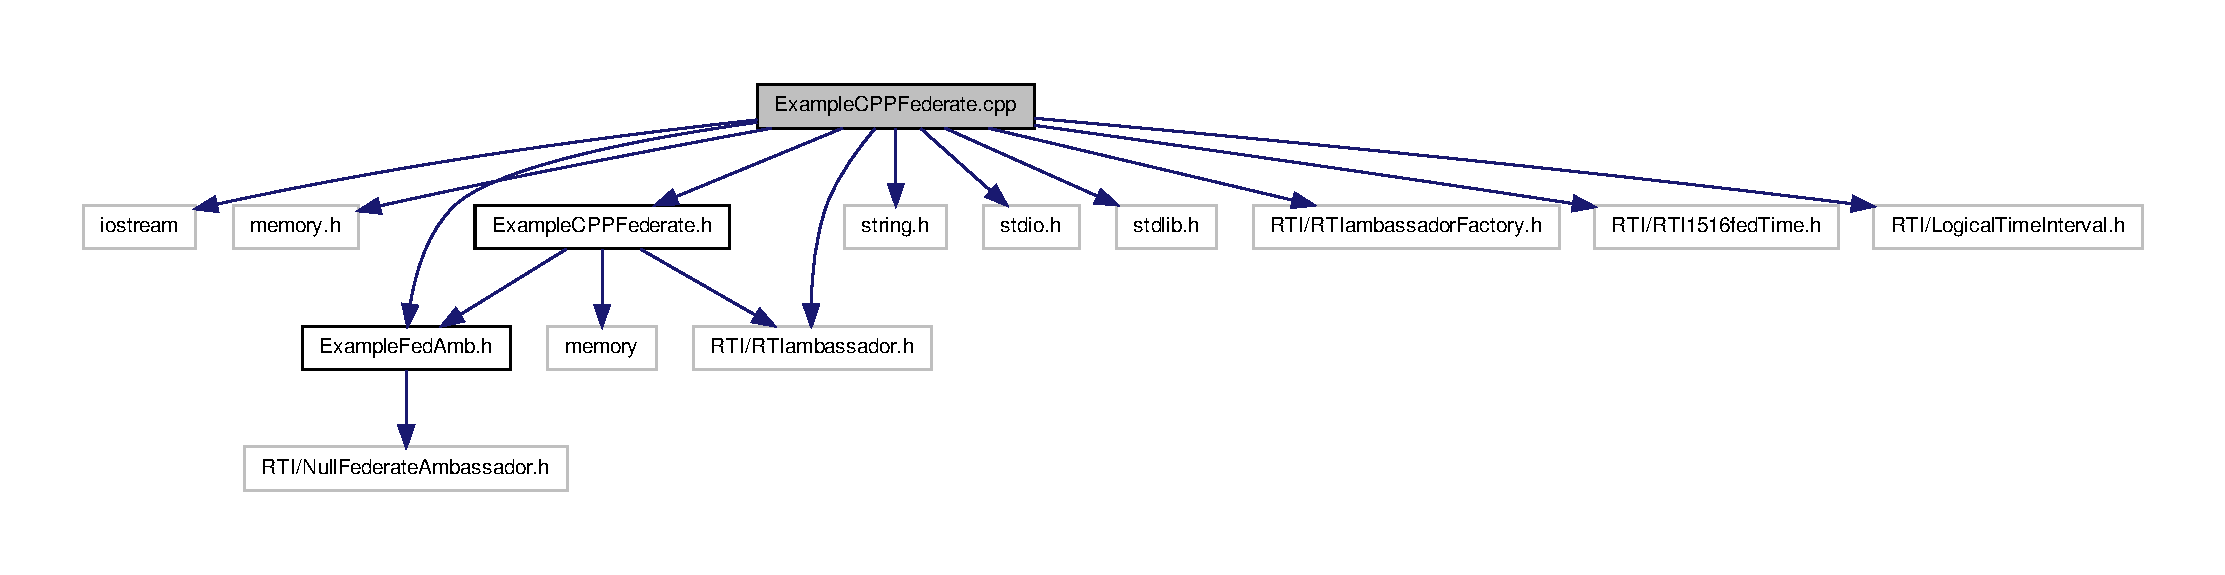
\includegraphics[width=400pt]{_example_c_p_p_federate_8cpp__incl}
\end{center}
\end{figure}


\subsection{Detailed Description}
Copyright (C) 2013 Max Oberberger $<$\href{mailto:max@oberbergers.de}{\tt max@oberbergers.de}$>$

Last modified: 2013 February 23, 20:05:02 by max

This file is part of ba-\/hla.

ba-\/hla is free software: you can redistribute it and/or modify it under the terms of the GNU General Public License as published by the Free Software Foundation, either version 3 of the License, or (at your option) any later version.

ba-\/hla is distributed in the hope that it will be useful, but WITHOUT ANY WARRANTY; without even the implied warranty of MERCHANTABILITY or FITNESS FOR A PARTICULAR PURPOSE. See the GNU General Public License for more details.

You should have received a copy of the GNU General Public License along with ba-\/hla. If not, see $<$\href{http://www.gnu.org/licenses/}{\tt http://www.gnu.org/licenses/}$>$. 